% Options for packages loaded elsewhere
\PassOptionsToPackage{unicode}{hyperref}
\PassOptionsToPackage{hyphens}{url}
\PassOptionsToPackage{dvipsnames,svgnames,x11names}{xcolor}
%
\documentclass[
  letterpaper,
  DIV=11,
  numbers=noendperiod]{scrartcl}

\usepackage{amsmath,amssymb}
\usepackage{iftex}
\ifPDFTeX
  \usepackage[T1]{fontenc}
  \usepackage[utf8]{inputenc}
  \usepackage{textcomp} % provide euro and other symbols
\else % if luatex or xetex
  \usepackage{unicode-math}
  \defaultfontfeatures{Scale=MatchLowercase}
  \defaultfontfeatures[\rmfamily]{Ligatures=TeX,Scale=1}
\fi
\usepackage{lmodern}
\ifPDFTeX\else  
    % xetex/luatex font selection
\fi
% Use upquote if available, for straight quotes in verbatim environments
\IfFileExists{upquote.sty}{\usepackage{upquote}}{}
\IfFileExists{microtype.sty}{% use microtype if available
  \usepackage[]{microtype}
  \UseMicrotypeSet[protrusion]{basicmath} % disable protrusion for tt fonts
}{}
\makeatletter
\@ifundefined{KOMAClassName}{% if non-KOMA class
  \IfFileExists{parskip.sty}{%
    \usepackage{parskip}
  }{% else
    \setlength{\parindent}{0pt}
    \setlength{\parskip}{6pt plus 2pt minus 1pt}}
}{% if KOMA class
  \KOMAoptions{parskip=half}}
\makeatother
\usepackage{xcolor}
\setlength{\emergencystretch}{3em} % prevent overfull lines
\setcounter{secnumdepth}{-\maxdimen} % remove section numbering
% Make \paragraph and \subparagraph free-standing
\ifx\paragraph\undefined\else
  \let\oldparagraph\paragraph
  \renewcommand{\paragraph}[1]{\oldparagraph{#1}\mbox{}}
\fi
\ifx\subparagraph\undefined\else
  \let\oldsubparagraph\subparagraph
  \renewcommand{\subparagraph}[1]{\oldsubparagraph{#1}\mbox{}}
\fi


\providecommand{\tightlist}{%
  \setlength{\itemsep}{0pt}\setlength{\parskip}{0pt}}\usepackage{longtable,booktabs,array}
\usepackage{calc} % for calculating minipage widths
% Correct order of tables after \paragraph or \subparagraph
\usepackage{etoolbox}
\makeatletter
\patchcmd\longtable{\par}{\if@noskipsec\mbox{}\fi\par}{}{}
\makeatother
% Allow footnotes in longtable head/foot
\IfFileExists{footnotehyper.sty}{\usepackage{footnotehyper}}{\usepackage{footnote}}
\makesavenoteenv{longtable}
\usepackage{graphicx}
\makeatletter
\def\maxwidth{\ifdim\Gin@nat@width>\linewidth\linewidth\else\Gin@nat@width\fi}
\def\maxheight{\ifdim\Gin@nat@height>\textheight\textheight\else\Gin@nat@height\fi}
\makeatother
% Scale images if necessary, so that they will not overflow the page
% margins by default, and it is still possible to overwrite the defaults
% using explicit options in \includegraphics[width, height, ...]{}
\setkeys{Gin}{width=\maxwidth,height=\maxheight,keepaspectratio}
% Set default figure placement to htbp
\makeatletter
\def\fps@figure{htbp}
\makeatother

\usepackage{fontspec}

\setsansfont{Palatino}[
    Path=/exam/final_exam/palatino/,
    Extension = .ttf,
    UprightFont=*-Roman,
    BoldFont=*-Bold,
    ItalicFont=*-Italic,
    BoldItalicFont=*-BoldItalic
]
\setmainfont{Palatino}

\usepackage[textwidth=0.86\paperwidth, textheight=0.86\paperheight]{geometry}
\usepackage{fancyhdr}
\usepackage{hyperref}
\usepackage{fontawesome5}
\usepackage{graphicx}
\usepackage{amssymb}
\usepackage{amsmath}

\newcommand{\R}{\mathbb{R}}

% \pagenumbering{gobble}
\pagestyle{fancy}
\fancyhead{} % clear all header fields
\fancyhead[R]{\href{https://mipt23.fmin.xyz}{\faGem[regular]} \hspace{0.04cm} \href{https://github.com/MerkulovDaniil/mipt23}{\faGithub} \hspace{0.07cm} \href{https://t.me/fminxyz}{\faTelegram}}
\fancyhead[L]{\href{https://fmin.xyz}{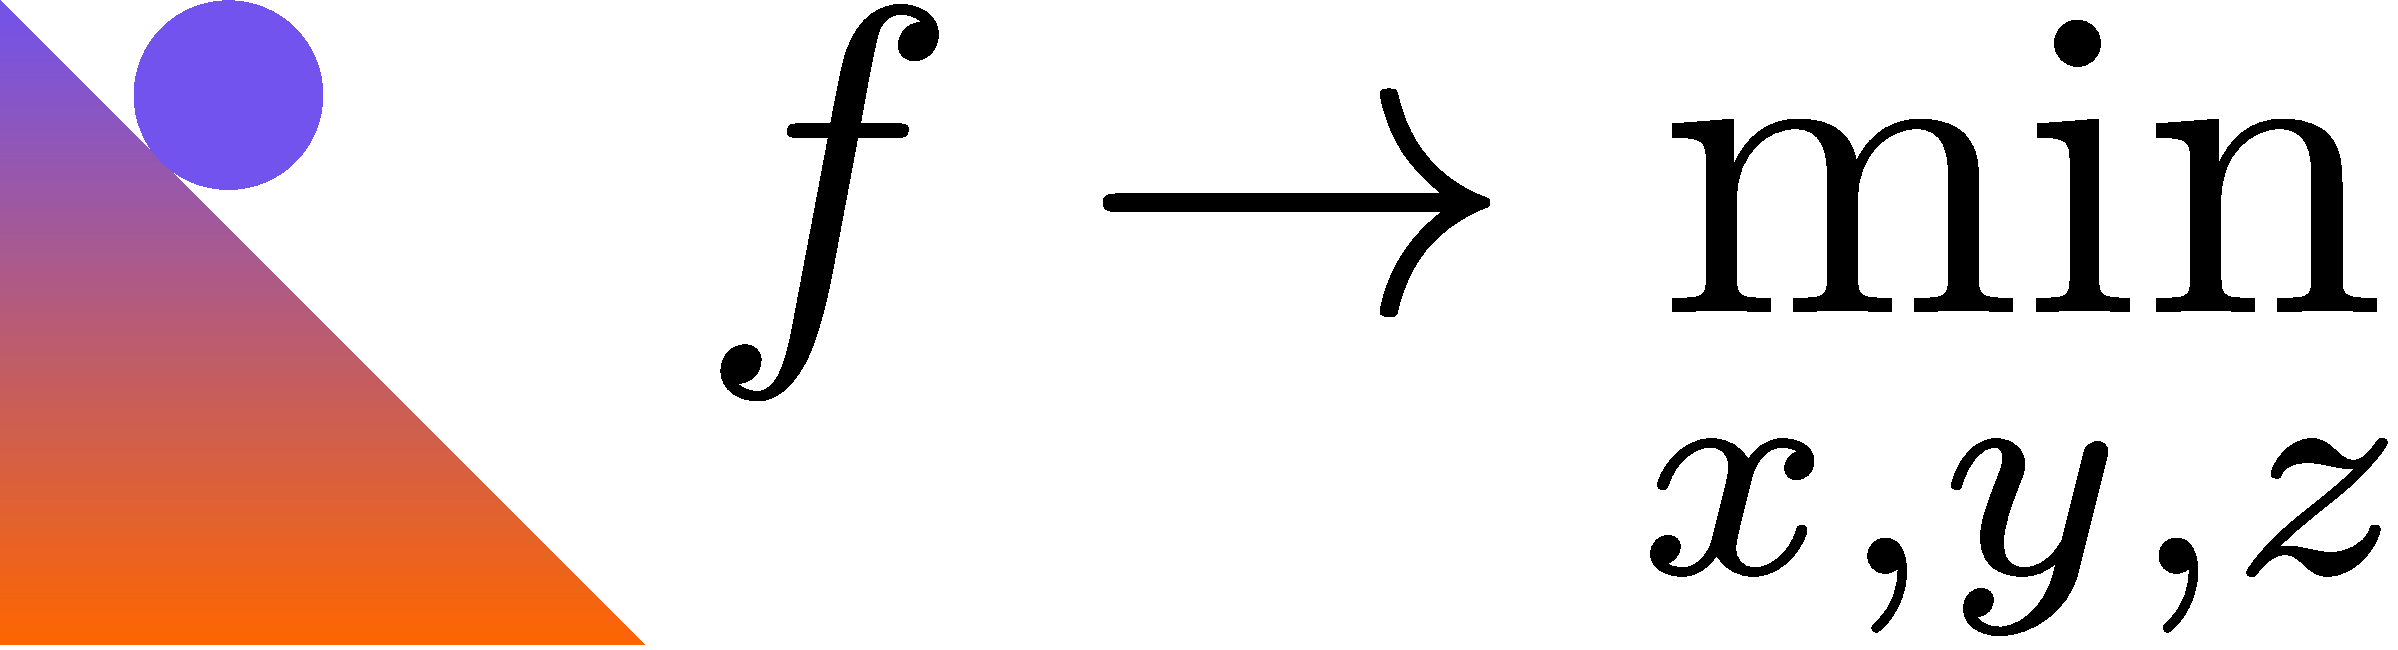
\includegraphics[height=0.35cm]{logo.pdf}} \hspace{2pt} \textbf{Методы оптимизации. МФТИ. 2024}}
\KOMAoption{captions}{tableheading}
\makeatletter
\@ifpackageloaded{caption}{}{\usepackage{caption}}
\AtBeginDocument{%
\ifdefined\contentsname
  \renewcommand*\contentsname{Table of contents}
\else
  \newcommand\contentsname{Table of contents}
\fi
\ifdefined\listfigurename
  \renewcommand*\listfigurename{List of Figures}
\else
  \newcommand\listfigurename{List of Figures}
\fi
\ifdefined\listtablename
  \renewcommand*\listtablename{List of Tables}
\else
  \newcommand\listtablename{List of Tables}
\fi
\ifdefined\figurename
  \renewcommand*\figurename{Figure}
\else
  \newcommand\figurename{Figure}
\fi
\ifdefined\tablename
  \renewcommand*\tablename{Table}
\else
  \newcommand\tablename{Table}
\fi
}
\@ifpackageloaded{float}{}{\usepackage{float}}
\floatstyle{ruled}
\@ifundefined{c@chapter}{\newfloat{codelisting}{h}{lop}}{\newfloat{codelisting}{h}{lop}[chapter]}
\floatname{codelisting}{Listing}
\newcommand*\listoflistings{\listof{codelisting}{List of Listings}}
\makeatother
\makeatletter
\makeatother
\makeatletter
\@ifpackageloaded{caption}{}{\usepackage{caption}}
\@ifpackageloaded{subcaption}{}{\usepackage{subcaption}}
\makeatother
\ifLuaTeX
  \usepackage{selnolig}  % disable illegal ligatures
\fi
\IfFileExists{bookmark.sty}{\usepackage{bookmark}}{\usepackage{hyperref}}
\IfFileExists{xurl.sty}{\usepackage{xurl}}{} % add URL line breaks if available
\urlstyle{same} % disable monospaced font for URLs
\hypersetup{
  colorlinks=true,
  linkcolor={blue},
  filecolor={Maroon},
  citecolor={Blue},
  urlcolor={Blue},
  pdfcreator={LaTeX via pandoc}}

\author{}
\date{}

\begin{document}
\section{Определения и
формулировки}\label{ux43eux43fux440ux435ux434ux435ux43bux435ux43dux438ux44f-ux438-ux444ux43eux440ux43cux443ux43bux438ux440ux43eux432ux43aux438}

\begin{enumerate}
\def\labelenumi{\arabic{enumi}.}
\tightlist
\item
  Показать, что направление антиградиента - направление наискорейшего
  локального убывания функции.
\item
  Метод градиентного спуска.
\item
  Наискорейший спуск.
\item
  Липшицева парабола для гладкой функции.
\item
  Размер шага наискорейшего спуска для квадратичной функции.
\item
  Характер сходимости градиентного спуска к локальному экстремуму для
  гладких невыпуклых функций в терминах \(\mathcal{O}\) от числа
  итераций метода.
\item
  Характер сходимости градиентного спуска для гладких выпуклых функций в
  терминах \(\mathcal{O}\) от числа итераций метода.
\item
  Характер сходимости градиентного спуска для гладких и сильно выпуклых
  функций в терминах \(\mathcal{O}\) от числа итераций метода.
\item
  Связь спектра гессиана с константами сильной выпуклости и гладкости
  функции.
\item
  Условие Поляка-Лоясиевича (градиентного доминирования) для функций.
\item
  Сходимость градиентного спуска для сильно выпуклых квадратичных
  функций. Оптимальные гиперпараметры.
\item
  Связь PL-функций и сильно выпуклых функций.
\item
  Привести пример выпуклой, но не сильно выпуклой задачи линейных
  наименьших квадратов (возможно, с регуляризацией).
\item
  Привести пример сильно выпуклой задачи линейных наименьших квадратов
  (возможно, с регуляризацией).
\item
  Привести пример выпуклой негладкой задачи линейных наименьших
  квадратов (возможно, с регуляризацией).
\item
  Субградиент. Субдифференциал.
\item
  Субградиентный метод.
\item
  Характер сходимости субградиентного метода для негладких выпуклых
  функций в терминах \(\mathcal{O}\) от числа итераций метода.
\item
  Нижние оценки для гладкой выпуклой оптимизации с помощью методов
  первого порядка в терминах \(\mathcal{O}\) от числа итераций метода.
\item
  Отличие ускоренной и неускоренной линейной сходимости для методов
  первого порядка.
\item
  Метод тяжелого шарика (Поляка).
\item
  Ускоренный градиентный метод Нестерова для выпуклых гладких функций.
\item
  Ускоренный градиентный метод Нестерова для сильно выпуклых гладких
  функций.
\item
  Проекция.
\item
  Достаточное условие существования проекции точки на множество.
\item
  Достаточное условие единственности проекции точки на множество.
\item
  Метод проекции градиента.
\item
  Критерий проекции точки на выпуклое множество (Неравенство
  Бурбаки-Чейни-Гольдштейна).
\item
  Проекция как нерастягивающий оператор.
\item
  Метод Франк-Вульфа.
\item
  Характер сходимости метода проекции градиента для гладких выпуклых
  функций в терминах \(\mathcal{O}\) от числа итераций метода.
\item
  Характер сходимости метода проекции градиента для гладких сильно
  выпуклых функций в терминах \(\mathcal{O}\) от числа итераций метода.
\item
  Характер сходимости метода Франк-Вульфа для гладких выпуклых функций в
  терминах \(\mathcal{O}\) от числа итераций метода.
\item
  Характер сходимости метода Франк-Вульфа для гладких сильно выпуклых
  функций в терминах \(\mathcal{O}\) от числа итераций метода.
\item
  \(A\)-сопряженность двух векторов. \(A\)-ортогональность. Скалярное
  произведение \(\langle \cdot, \cdot \rangle_A\).
\item
  Процедура ортогонализации Грама-Шмидта.
\item
  Метод сопряженных направлений.
\item
  Метод сопряженных градиентов.
\item
  Зависимость сходимости метода сопряженных градиентнов от спектра
  матрицы.
\item
  Характер сходимости метода сопряженных градиентов в терминах
  \(\mathcal{O}\) от числа итераций метода.
\item
  Метод Поляка-Рибьера.
\item
  Метод Ньютона.
\item
  Сходимость метода Ньютона для квадратичной функции.
\item
  Характер сходимости метода Ньютона для сильно выпуклых гладких функций
  - куда и как сходится.
\item
  Демпфированный метод Ньютона.
\item
  Идея квазиньютоновских методов. Метод SR-1.
\item
  Нижние оценки для негладкой выпуклой оптимизации с помощью методов
  первого порядка в терминах \(\mathcal{O}\) от числа итераций метода.
\item
  Проксимальный оператор.
\item
  Оператор проекции как частный случай проксимального оператора.
\item
  Характер сходимости проксимального градиентного метода для гладких
  выпуклых функций \(f\) в терминах \(\mathcal{O}\) от числа итераций
  метода.
\item
  Характер сходимости проксимального градиентного метода для гладких
  сильно выпуклых функций \(f\) в терминах \(\mathcal{O}\) от числа
  итераций метода.
\item
  Аналитическое выражение для \(\text{prox}_{\lambda \|x\|_1}\).
\item
  Аналитическое выражение для \(\text{prox}_{\frac{\mu}{2} \|x\|_2^2}\).
\item
  Проксимальный оператор как нерастягивающий оператор.
\item
  Характер сходимости ускоренного проксимального градиентного метода для
  гладких выпуклых функций \(f\) в терминах \(\mathcal{O}\) от числа
  итераций метода.
\item
  Метод стохастического градиентного спуска.
\item
  Идея мини-батча для метода стохастического градиентного спуска. Эпоха.
\item
  Характер сходимости стохастического градиентного спуска для гладких
  выпуклых функций в терминах \(\mathcal{O}\) от числа итераций метода.
\item
  Характер сходимости стохастического градиентного спуска для гладких
  PL-функций в терминах \(\mathcal{O}\) от числа итераций метода.
\item
  Характер работы стохастического градиентного спуска с постоянным шагом
  для гладких PL-функций.
\item
  Основная идея методов уменьшения дисперсии.
\item
  Метод SVRG.
\item
  Метод SAG.
\item
  Метод Adagrad.
\item
  Метод RMSProp.
\item
  Метод Adadelta.
\item
  Метод Adam.
\item
  Идея проекции функции потерь нейронной сети на прямую, плоскость.
\item
  Grokking.
\item
  Double Descent.
\item
  Взрыв/Затухание градиентов при обучении глубоких нейронных сетей.
\item
  Идея gradient checkpointing.
\item
  Идея аккумуляции градиентов.
\item
  Зачем увеличивать батч при обучении больших нейросетевых моделей.
  Warmup.
\item
  Дифференциальное уравнение градиентного потока.
\item
  Характер сходимости траектории градиентного потока для выпуклых
  функций в терминах \(\mathcal{O}\left( t \right)\).
\item
  Характер сходимости траектории градиентного потока для PL-функций в
  терминах \(\mathcal{O}\left( t \right)\).
\item
  Дифференциальное уравнение Нестеровского ускоренного градиентного
  потока.
\item
  Метод двойственного градиентного подъема.
\item
  Связь константы сильной выпуклости \(f\) и гладкости \(f^*\).
\item
  Идея dual decomposition.
\item
  Метод двойственного градиентного подъема для линейных
  ограничений-неравенств.
\item
  Метод модифицированной функции Лагранжа.
\item
  Метод ADMM.
\item
  Формулировка задачи линейных наименьших квадратов с \(\ell_1\)
  регуляризацией в форме ADMM.
\item
  Формулировка задачи поиска точки на пересечении двух выпуклых множеств
  в форме ADMM.
\end{enumerate}

\section{Теоремы с
доказательствами}\label{ux442ux435ux43eux440ux435ux43cux44b-ux441-ux434ux43eux43aux430ux437ux430ux442ux435ux43bux44cux441ux442ux432ux430ux43cux438}

\begin{enumerate}
\def\labelenumi{\arabic{enumi}.}
\tightlist
\item
  Теорема сходимости градиентного спуска для гладких выпуклых функций.
\item
  Теорема сходимости градиентного спуска для гладких PL функций.
\item
  Теорема сходимости градиентного спуска для сильно выпуклых
  квадратичных функций. Оптимальные гиперпараметры.
\item
  Теорема сходимости субградиентного метода для выпуклых функций.
  Сходимость метода для разных стратегий выбора шага: постоянный размер
  шага \(\alpha_k = \alpha\); Обратный квадратный корень
  \(\frac{R}{G\sqrt{k}}\); Обратный \(\frac1k\); Размер шага Поляка:
  \(\alpha_k = \frac{f(x^k) - f^*}{\|g_k\|_2^2}\).
\item
  Теорема о сходимости метода тяжелого шарика для сильно выпуклой
  квадратичной задачи.
\item
  Теорема о сходимости метода проекции градиента для выпуклой гладкой
  функции.
\item
  Теорема о сходимости метода проекции градиента для сильно выпуклой
  гладкой функции.
\item
  Теорема о сходимости метода Франк-Вульфа для выпуклой гладкой функции.
\item
  Доказательство сходимости метода сопряженных градиентов и вывод
  формулы.
\item
  Теорема сходимости метода Ньютона для сильно выпуклых функций с
  липшицевым гессианом.
\item
  Вывод формул обновления оценок обратного гессиана и гессиана
  квазиньютоновских методов SR-1, DFP, BFGS.
\item
  Теорема о сходимости проксимального градиентного для выпуклой гладкой
  функции \(f\).
\item
  Теорема о сходимости проксимального градиентного для сильно выпуклой
  гладкой функции \(f\).
\item
  Теорема о сходимости стохастического градиентного спуска в гладком
  PL-случае.
\item
  Теорема сходимости траектории градиентного потока для выпуклых и
  PL-функций.
\end{enumerate}

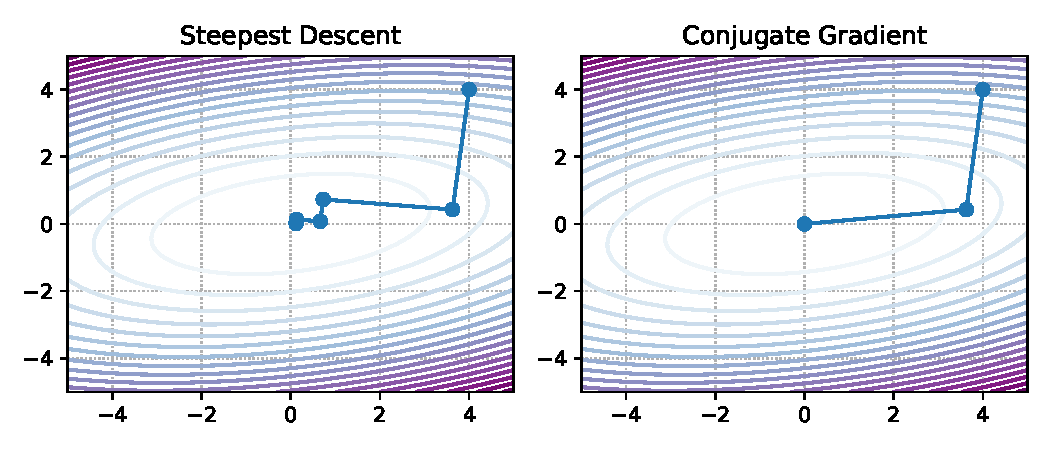
\includegraphics[width=0.94\textwidth,height=\textheight]{SD_vs_CG.pdf}



\end{document}
